% day02.tex

% Editing Author: Mason del Rosario 
% Description: A modified version of Pavillet's Oxonion template for UC Davis

% Copyright 2019 Clara Eleonore Pavillet

% Author: Clara Eleonore Pavillet
% Description: This is an unofficial Oxford University Beamer Template I made from scratch. Feel free to use it, modify it, share it.
% Version: 1.0

\documentclass{beamer}
\setbeamertemplate{caption}[numbered]
\usepackage{import} % for some reason, this doesn't work when called in sty file
% Load Packages
\usepackage[utf8]{inputenc}
\usepackage{xcolor}
\usepackage{tikz}
\usetikzlibrary{positioning,calc}
\usepackage{graphicx}
\usepackage{hyperref}
\usepackage{amsmath}
\usepackage{listings}
\usepackage{fontawesome}

% Define Commands
\newcommand*{\ClipSep}{0.06cm} %To adjust footer logo
\newcommand{\E}{\mathrm{e}\,} %\def\I{e} % used to defined e for exp(x), see later what it should be
\newcommand{\ud}{\mathrm{d}}
\lstset{numbers=left, numberstyle=\tiny, stepnumber=1,firstnumber=1,breaklines=true,
    numbersep=5pt,language=Python,
    stringstyle=\ttfamily,
    basicstyle=\footnotesize, 
    showstringspaces=false
}

\usepackage{lecture_notes}
\usepackage{bibentry}
\usepackage[utf8]{inputenc}
\usepackage[T1]{fontenc}

% for manual multicolumns
\usepackage{multicol}
\setlength{\columnseprule}{1pt}
\def\columnseprulecolor{\color{black}}

% for embedded code (i.e., .bib reference)
\usepackage{listings}

\graphicspath{ {../../images/} }

\nobibliography*
% \usepackage[perpage]{footmisc}
\usetheme{oxonian}


\title{Day 02: Intro to \LaTeX}
\titlegraphic{
\includegraphics[width=3cm]{Theme/Logos/DavisLogoV1.png}}
\author{\small{Mason del Rosario}}
\institute{\LaTeX 101}
\date{March 22, 2022} %\today

\begin{document}

\footnotesize{
% \bibliographystyle{ieeetr}
% \nobibliography*{refs}


{\setbeamertemplate{footline}{} 
\frame{\titlepage}}

  \section*{Course Recap}

  \begin{frame}{Course Recap}
    \begin{itemize} 
      \item \textbf{Adapted from} -- https://www.learnlatex.org/. 
        \begin{itemize}
          \item Day 1 -- \texttt{learnlatex.org} lessons 1-6 (\textbf{Done!})
          \item Day 2 -- \texttt{learnlatex.org} lessons 7-12.
          \item Day 3 -- Specific templates (resume, presentations).
        \end{itemize}
      \item \textbf{Slides Available} -- https://github.com/mdelrosa/latex-101.
      \begin{itemize}
        \item Template based on \href{https://www.overleaf.com/latex/templates/oxpav/xnjgrxthvjhg}{Clara Pavillet's Oxford Template}
      \end{itemize}
      \item \textbf{Slack back channel}
      \begin{itemize}
        \item \href{https://join.slack.com/share/zt-ul82okyc-SI2GftuwPx_lFyBXll9rjw}{UC Davis Slack channel}
      \end{itemize}
    \end{itemize}
  \end{frame}

  \section*{Outline}\begin{frame}{Outline}\tableofcontents\end{frame}

  \section{Figures}

  \begin{frame}[plain]
    \vfill
    \centering
    \begin{beamercolorbox}[sep=8pt,center,shadow=true,rounded=true]{Graphics}
      \usebeamerfont{title}\insertsectionhead\par%
      \color{davisblue}\noindent\rule{10cm}{1pt} \\
      \footnotesize{Including images, resizing, positioning}
    \end{beamercolorbox}
    \vfill
  \end{frame}

  \begin{frame}{\texttt{graphicx} package}
    The \texttt{graphicx} package provides the \texttt{\textbackslash includegraphics} command.
    \begin{figure}
      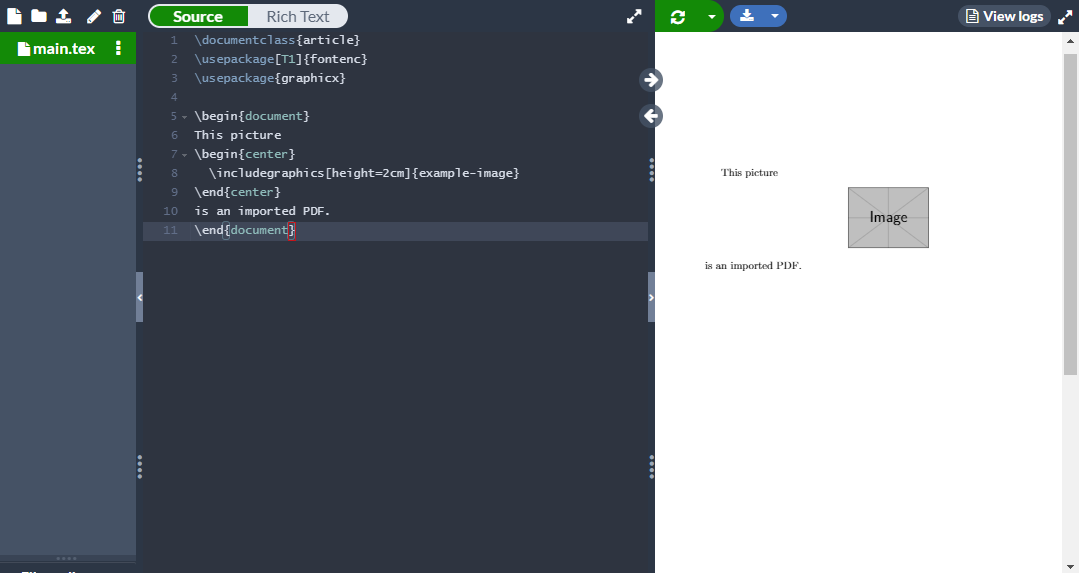
\includegraphics[width=0.9\linewidth]{day01-overleaf-10A-graphic.png}
      \caption{\texttt{example-image} is provided by default in most \LaTeX distributions.}
      \label{fig:day01-overleaf-10A}
    \end{figure}
  \end{frame}

  \nofoot{
  \begin{frame}{Scaling Images}
    \begin{itemize} 
      \item \texttt{\textbackslash includegraphics} takes optional arguments for scaling
      \item Common commands: \texttt{\textbackslash textheight}, \texttt{\textbackslash textwidth}
    \end{itemize}
    \begin{figure}
      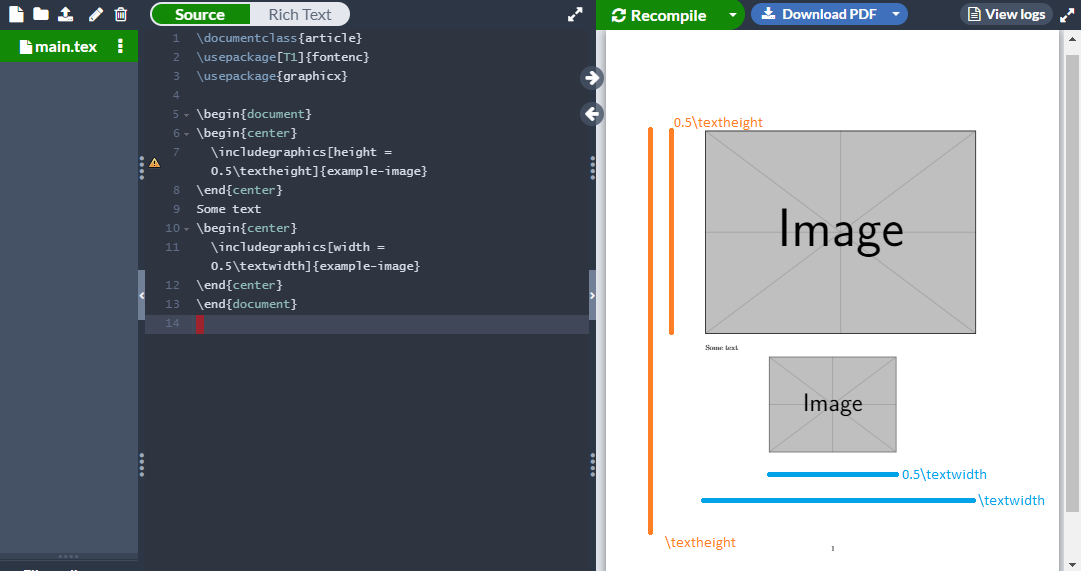
\includegraphics[width=0.9\linewidth]{day01-overleaf-10B-graphic.png}
      \caption{Optional arguments to change \texttt{width} and \texttt{height} of graphics.}
      \label{fig:day01-overleaf-10B}
    \end{figure}
  \end{frame}
  }

  \nofoot{
  \begin{frame}{Clipping, Rotating Images}
    \texttt{\textbackslash includegraphics} takes optional arguments for clipping and rotating
    \begin{figure}
      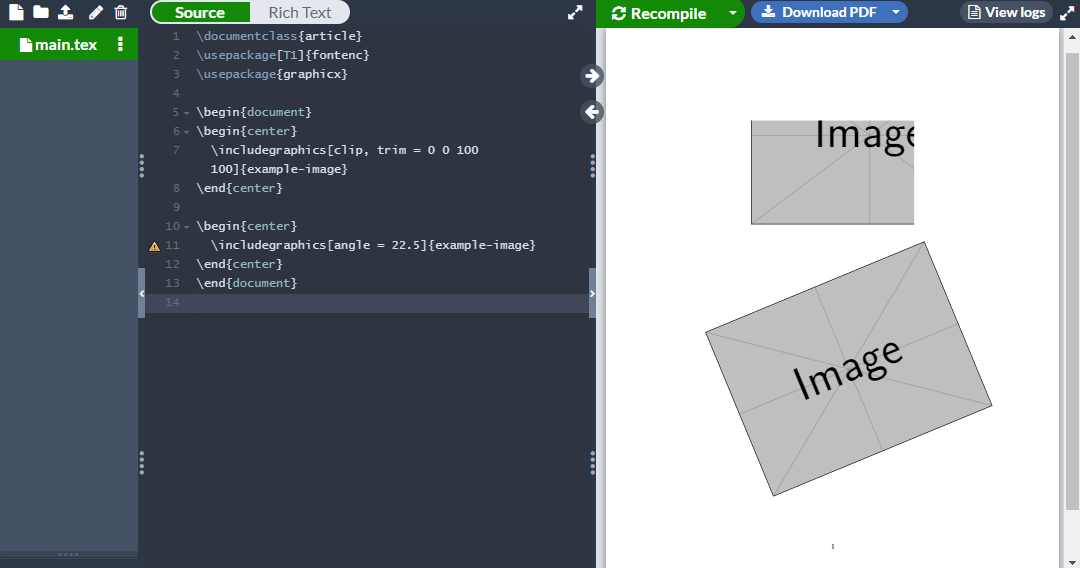
\includegraphics[width=0.9\linewidth]{day01-overleaf-10C-graphic.png}
      \caption{Optional arguments \texttt{clip}, \texttt{trim}, and \texttt{angle}.}
      \label{fig:day01-overleaf-10C}
    \end{figure}
  \end{frame}
  }

  \nofoot{
  \begin{frame}{Floats}
    Including images can lead to large gaps in text.
    \begin{figure}
      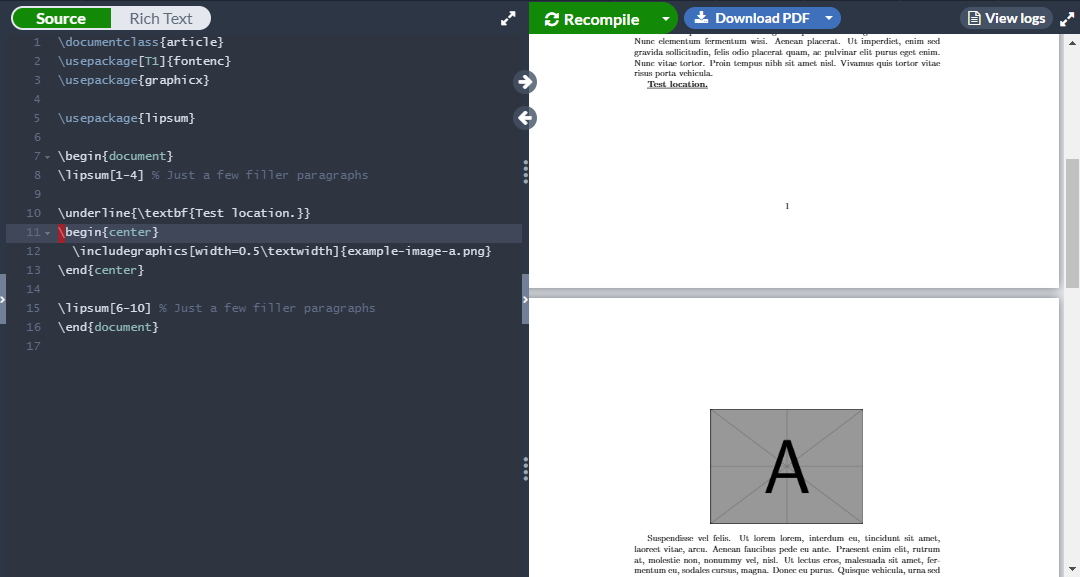
\includegraphics[width=0.9\linewidth]{day01-overleaf-10D-graphic.png}
      \caption{\texttt{\textbackslash includegraphics} causing a gap on Page 1}.
      \label{fig:day01-overleaf-10D}
    \end{figure}
  \end{frame}
  }

  \nofoot{
  \begin{frame}{Floats}
    \underline{Floats} - an image environment (e.g., \texttt{figure}) that dynamically adjusts its position.
    \begin{figure}
      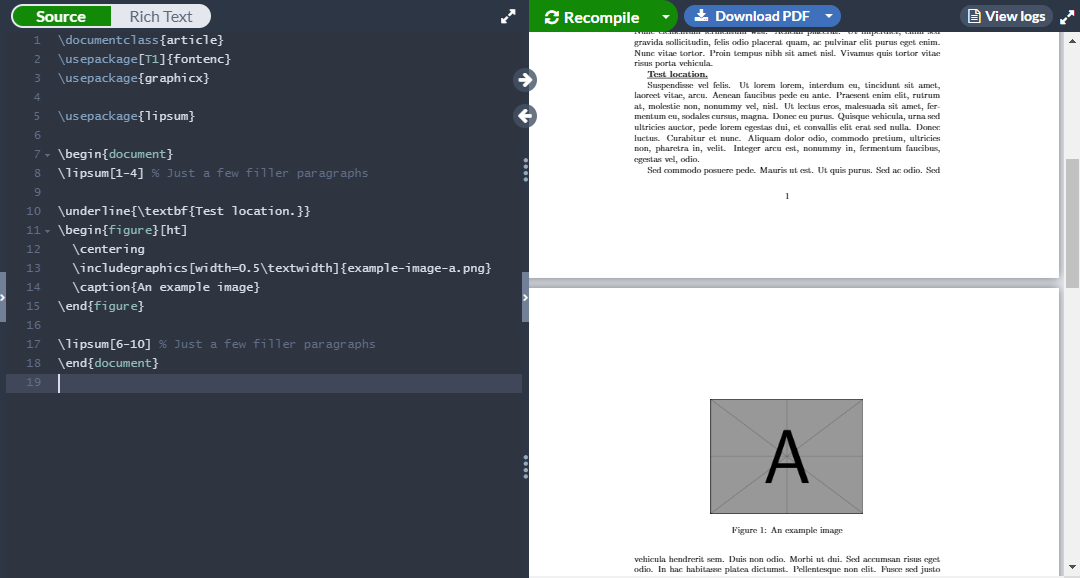
\includegraphics[width=0.9\linewidth]{day01-overleaf-10E-graphic-float.png}
      \caption{\texttt{figure} environment causes text to wrap properly}.
      \label{fig:day01-overleaf-10E}
    \end{figure}
  \end{frame}
  }

  \nofoot{
  \begin{frame}{Floats}
    Optional arguments \texttt{[h]}ere, \texttt{[t]}op, \texttt{[b]}ottom, \texttt{[p]}age control float placement.
    \begin{figure}
      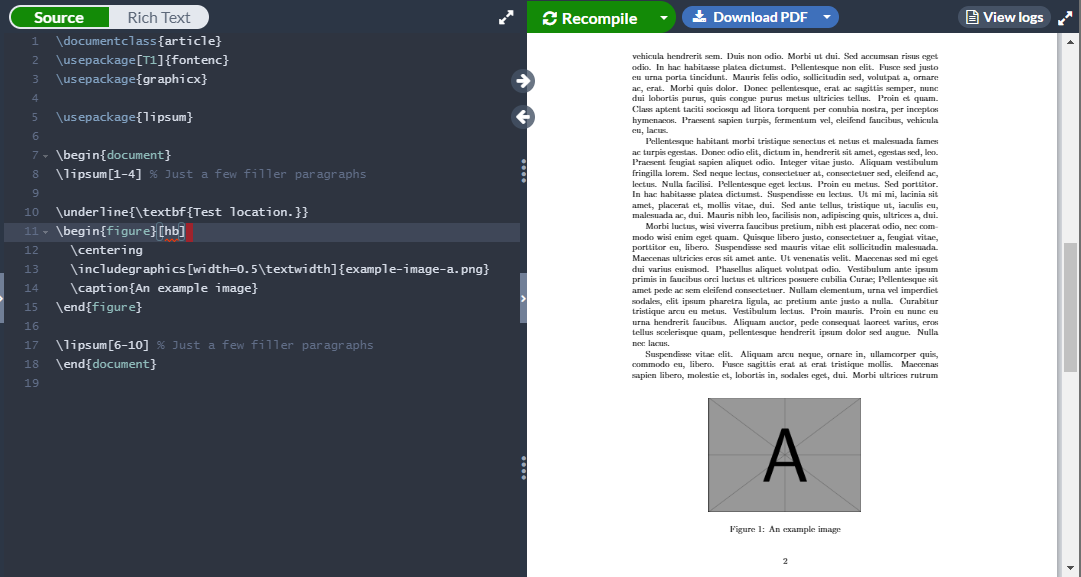
\includegraphics[width=0.9\linewidth]{day01-overleaf-10F-graphic-float.png}
      \caption{\texttt{figure} with \texttt{[hb]} optional argument placed on bottom of page}.
      \label{fig:day01-overleaf-10F}
    \end{figure}
  \end{frame}
  }

  \section{Tables}

  \begin{frame}[plain]
    \vfill
    \centering
    \begin{beamercolorbox}[sep=8pt,center,shadow=true,rounded=true]{Tables}
      \usebeamerfont{title}\insertsectionhead\par%
      \color{davisblue}\noindent\rule{10cm}{1pt} \\
      \footnotesize{Building tables, aligning and merging cells}
    \end{beamercolorbox}
    \vfill
  \end{frame}

  \begin{frame}{\texttt{array} package}
    The \texttt{array} package provides commands for tables.
    \begin{figure}
      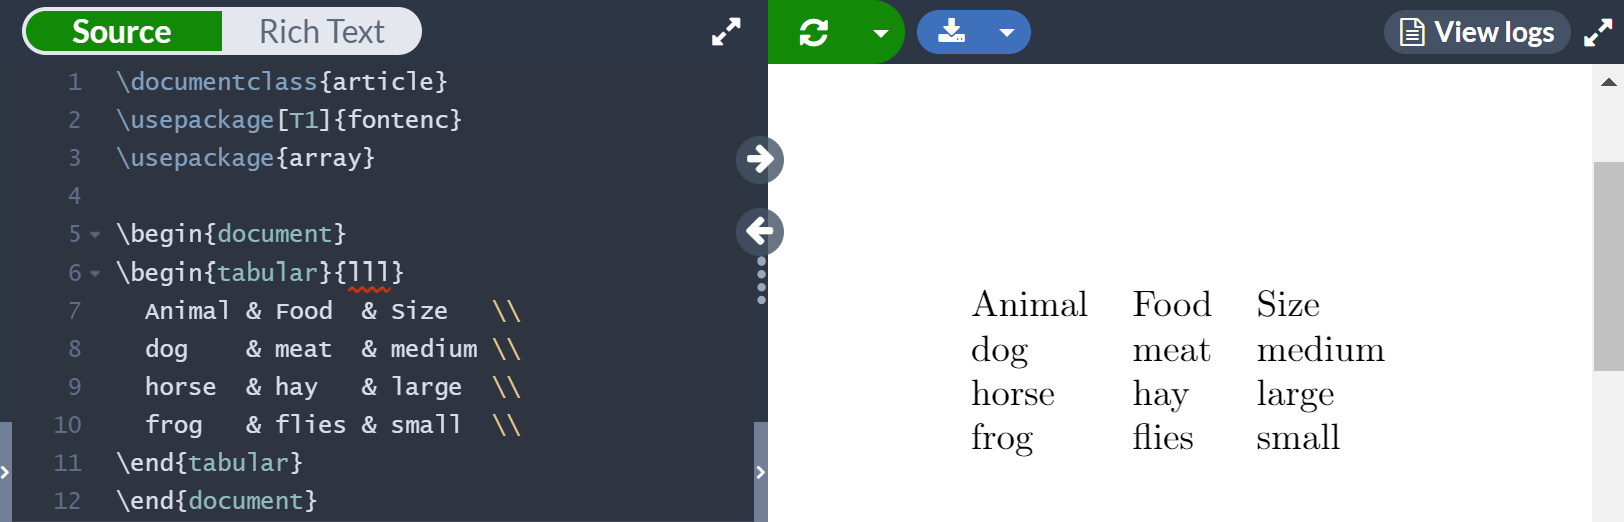
\includegraphics[width=0.9\linewidth]{day01-overleaf-11A-table.png}
      \caption{A \texttt{tabular} environment provided by \texttt{array} packages.}
      \label{fig:day01-overleaf-11A}
    \end{figure}
  \end{frame}

  \begin{frame}{Aligning Columns}
    Argument to \texttt{tabular} changes alignment -- \texttt{\{l\}}eft, \texttt{\{c\}}enter, \texttt{\{r\}}ight.
    \begin{figure}
      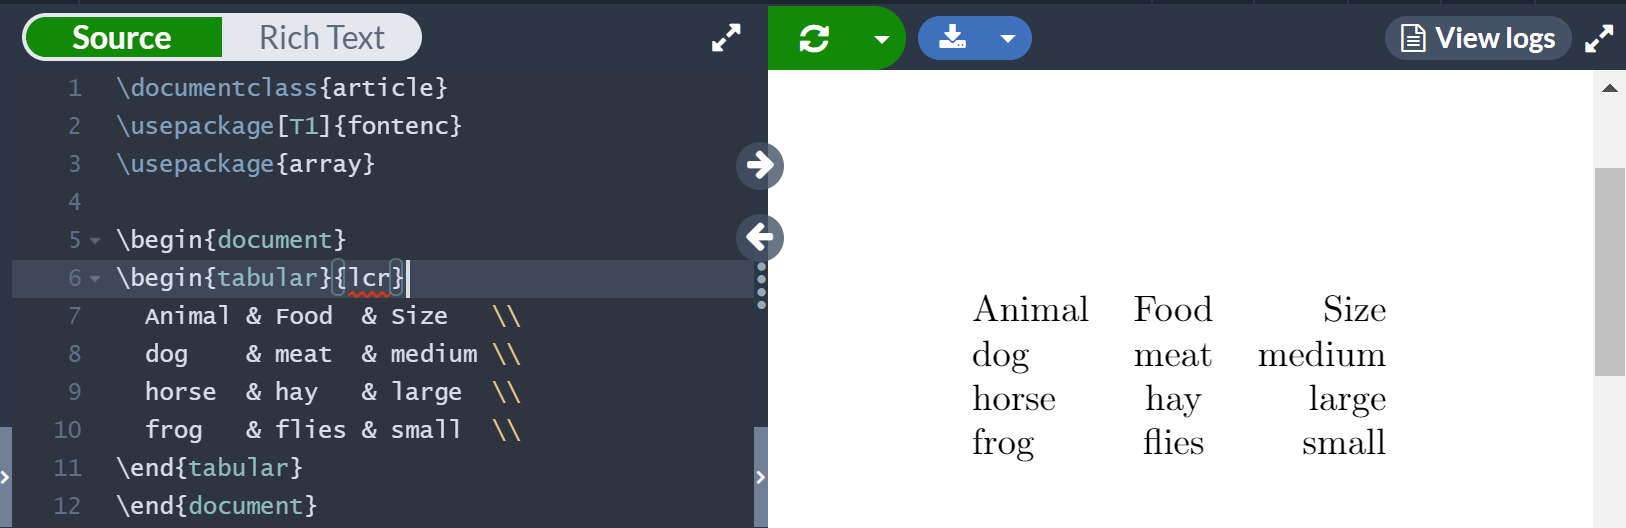
\includegraphics[width=0.9\linewidth]{day01-overleaf-11B-table-align.png}
      \caption{Same table with left, center, and right (\texttt{\{lcr\}}) column alignments.}
      \label{fig:day01-overleaf-11B}
    \end{figure}
  \end{frame}

  \begin{frame}{Paragraph Columns}
    (\texttt{\{lcr\}}) columns will typeset into single row, even if they are wider than the page.
    \begin{figure}
      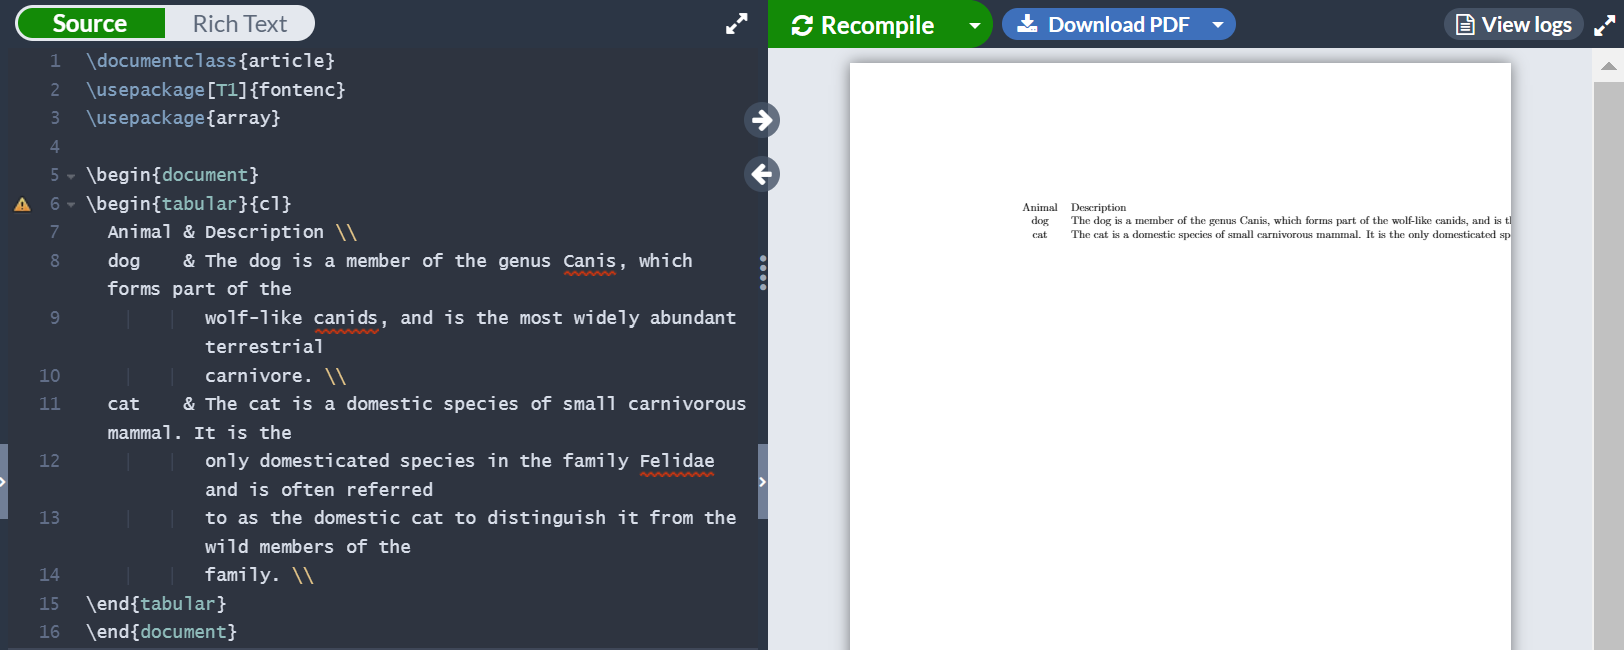
\includegraphics[width=0.9\linewidth]{day01-overleaf-11C-table-overflow.png}
      \caption{A runaway \texttt{l} column.}
      \label{fig:day01-overleaf-11C}
    \end{figure}
  \end{frame}

  \begin{frame}{Paragraph Columns}
    (\texttt{\{p\}}) columns are forced to a given width.
    \begin{figure}
      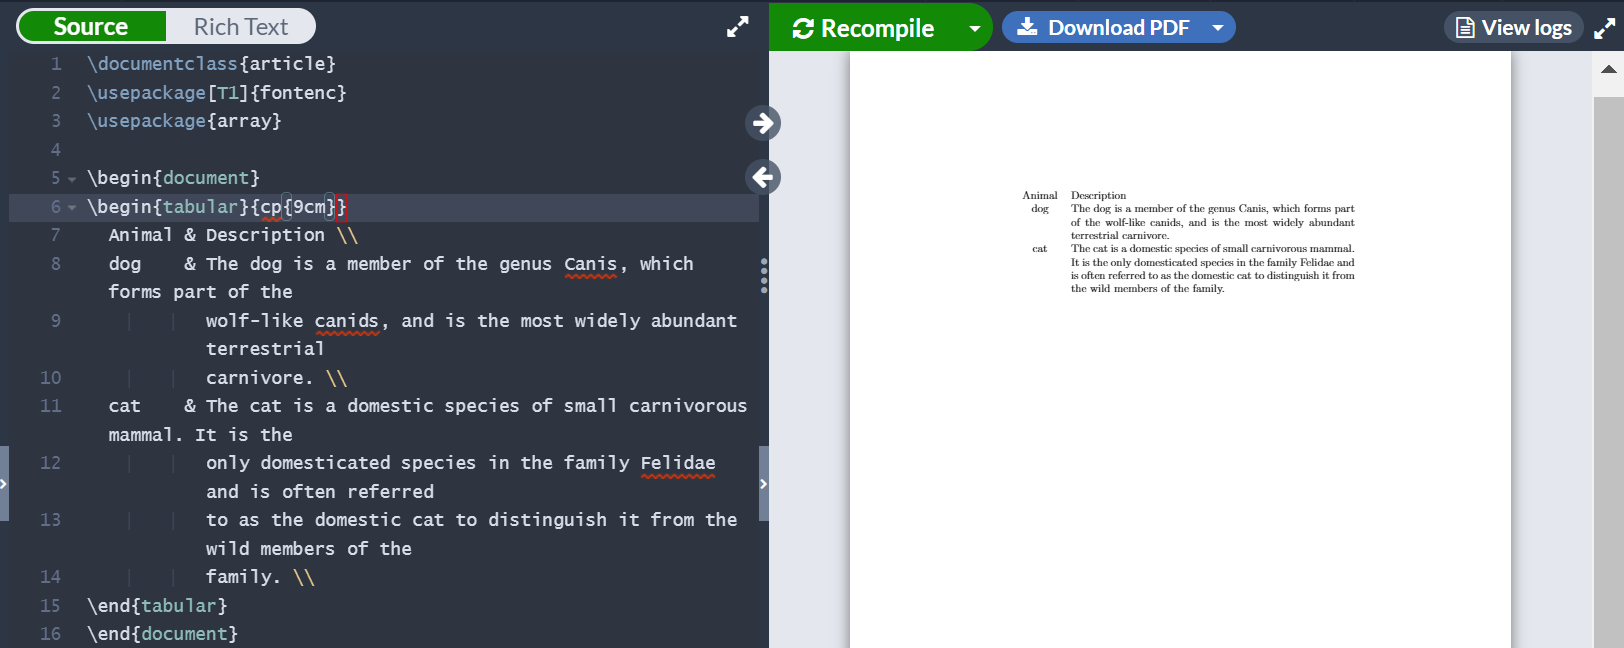
\includegraphics[width=0.9\linewidth]{day01-overleaf-11D-table-overflow.png}
      \caption{Same text in a \texttt{p} column with wrapped text.}
      \label{fig:day01-overleaf-11D}
    \end{figure}
  \end{frame}

  \begin{frame}{Adding rules}
    Rules (lines) are enabled with the \texttt{booktabs} package.
    \begin{figure}
      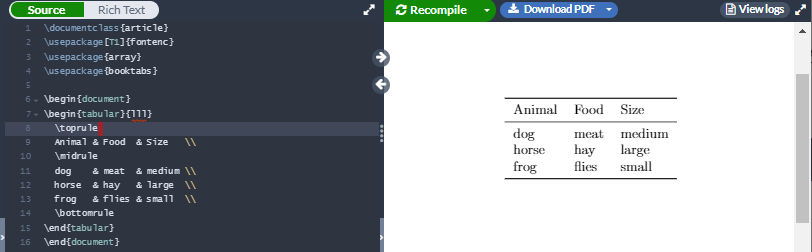
\includegraphics[width=0.9\linewidth]{day01-overleaf-11E-table-rule.png}
      % \caption{}
      % \label{fig:day01-overleaf-11E}
    \end{figure}
  \end{frame}

  \begin{frame}{Adding rules}
    \texttt{\textbackslash cmidrule} spans a subset of columns.
    \begin{figure}
      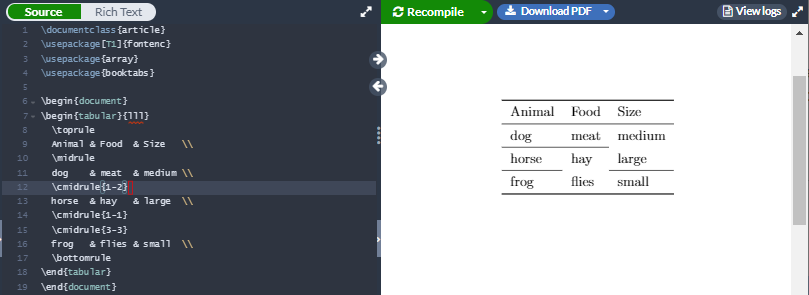
\includegraphics[width=0.9\linewidth]{day01-overleaf-11F-table-cmidrule.png}
    \end{figure}
  \end{frame}

  \begin{frame}{Adding line space}
    \texttt{\textbackslash addlinespace} useful for more subtle separation.
    \begin{figure}
      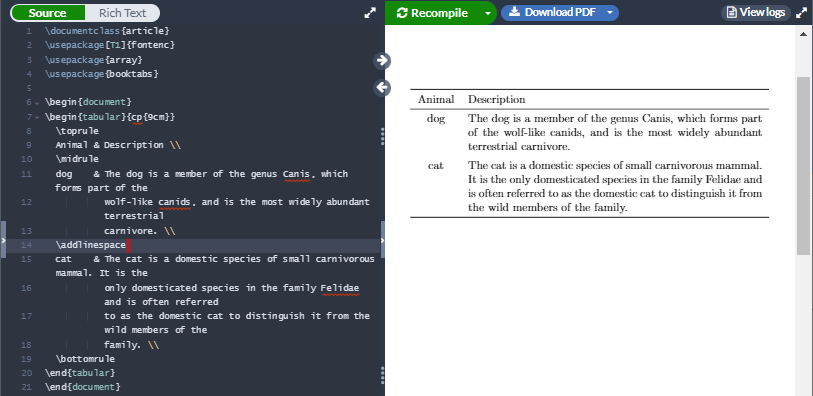
\includegraphics[width=0.9\linewidth]{day01-overleaf-11G-table-linespace.png}
    \end{figure}
  \end{frame}

  \begin{frame}{Merging cells}
    \texttt{\textbackslash multicolumn} creates cells spanning multiple columns. Arguments include:
    \begin{enumerate}
      \item Number of columns cell spans
      \item Alignment of cell
      \item Contents of cell
    \end{enumerate}
    \begin{figure}
      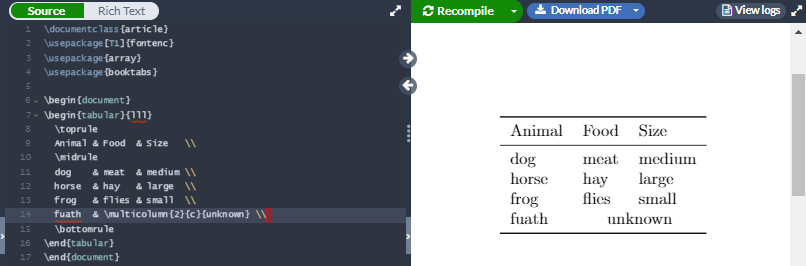
\includegraphics[width=0.9\linewidth]{day01-overleaf-11H-table-merge.png}
    \end{figure}
  \end{frame}

  \begin{frame}{Merging cells vertically}
    \texttt{multirow} package exists, but you can just use blank cells!
    \begin{figure}
      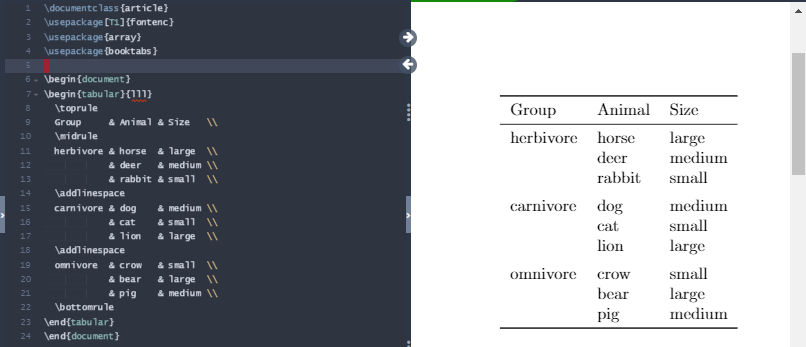
\includegraphics[width=0.9\linewidth]{day01-overleaf-11I-table-vertmerge.png}
    \end{figure}
  \end{frame}

  \nofoot{
  \begin{frame}{Table Generation}
    Useful utility for table creation: \url{https://www.tablesgenerator.com/}.
    \begin{figure}
      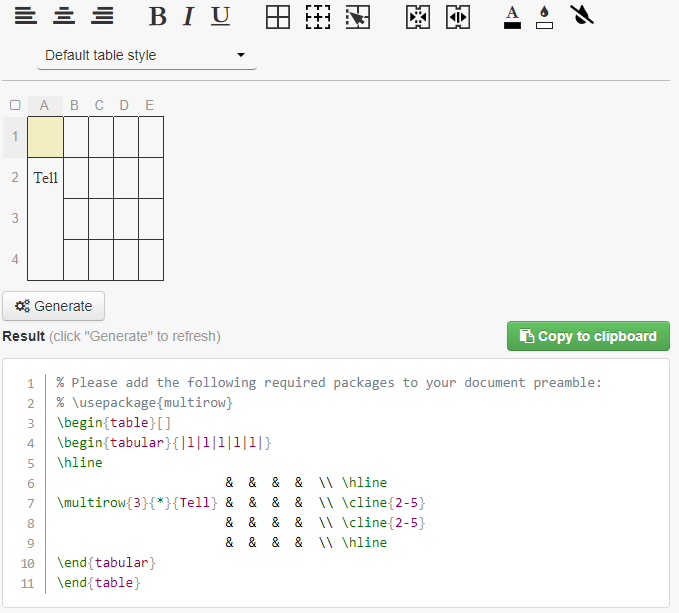
\includegraphics[width=0.6\linewidth]{day01-overleaf-12A-table-creation.png}
      \caption{Generate code for table based on WYSIWYG editor.}
      \label{fig:day01-overleaf-12A}
    \end{figure}
  \end{frame}
  }

  %TODO: potentially add interactive section for tablesgenerator?
  % e.g., "try generating some LaTeX code for a complicated table. do any unfamiliar commands pop up?"

  \section{Cross Referencing}

  \begin{frame}[plain]
    \vfill
    \centering
    \begin{beamercolorbox}[sep=8pt,center,shadow=true,rounded=true]{Cross Referencing}
      \usebeamerfont{title}\insertsectionhead\par%
      \color{davisblue}\noindent\rule{10cm}{1pt} \\
      \footnotesize{Smart references for figures, tables, sections, etc.}
    \end{beamercolorbox}
    \vfill
  \end{frame}

  \begin{frame}{\texttt{\textbackslash label} and \texttt{\textbackslash ref}}
    \begin{itemize}
      \item \texttt{\textbackslash label} commands assign ID to the most recent numbered element.
      \item \texttt{\textbackslash ref} commands display number corresponding to label with same ID.
    \end{itemize}
    \begin{figure}
      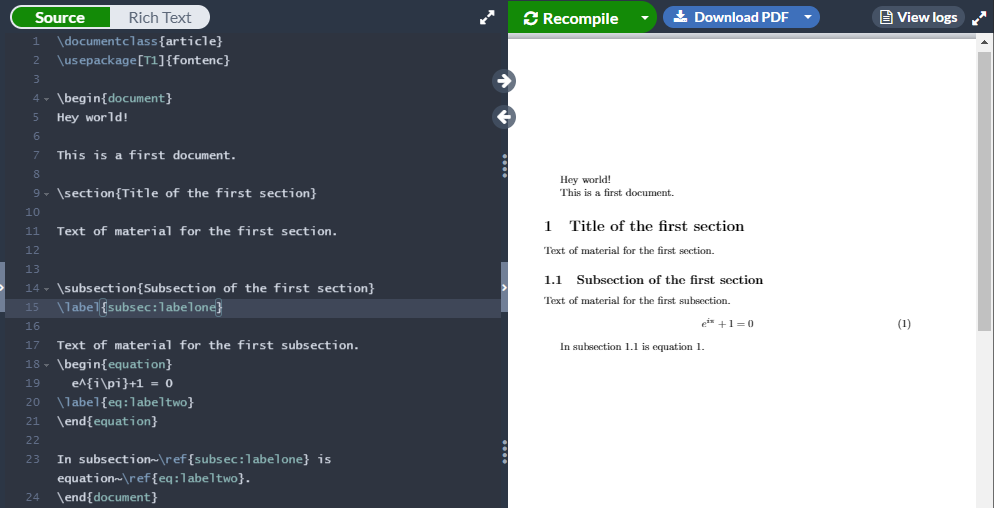
\includegraphics[width=0.9\linewidth]{day02-00A-references.png}
      \caption{\texttt{\textbackslash label} and \texttt{ref} commands used to number \texttt{section} and \texttt{equation} environments.}
      \label{fig:day02-00A}
    \end{figure}
  \end{frame}

  \begin{frame}{Naming conventions}
    \texttt{\textbackslash label} and \texttt{\textbackslash ref} accept any text as arguments.

    Good to name labels after corresponding elements, for example:
    \begin{itemize}
      \item \texttt{\textbackslash label\{eq:...\}} for equations
      \item \texttt{\textbackslash label\{sec:...\}} for sections
      \item \texttt{\textbackslash label\{tab:...\}} for tables
    \end{itemize}
  \end{frame}

  \section{Mathematics}

  \begin{frame}[plain]
    \vfill
    \centering
    \begin{beamercolorbox}[sep=8pt,center,shadow=true,rounded=true]{Mathematics}
      \usebeamerfont{title}\insertsectionhead\par%
      \color{davisblue}\noindent\rule{10cm}{1pt} \\
      \footnotesize{Inline vs. display equations}
    \end{beamercolorbox}
    \vfill
  \end{frame}

  \begin{frame}{Inline vs. Display Equations}
    \LaTeX's biggest feature: \emph{math mode}. Two categories of math mode equations:
    \begin{enumerate}
      \item \textbf{Inline}: Does not break paragraph. Denoted by $\$\dots\$$ or \textbackslash$(\dots$\textbackslash$)$.
      \item \textbf{Display}: Breaks paragraph, centers equation. Denoted by \textbackslash$[\dots$\textbackslash$]$, \texttt{equation} environment, or \texttt{align} environment.
    \end{enumerate}
    \begin{figure}
      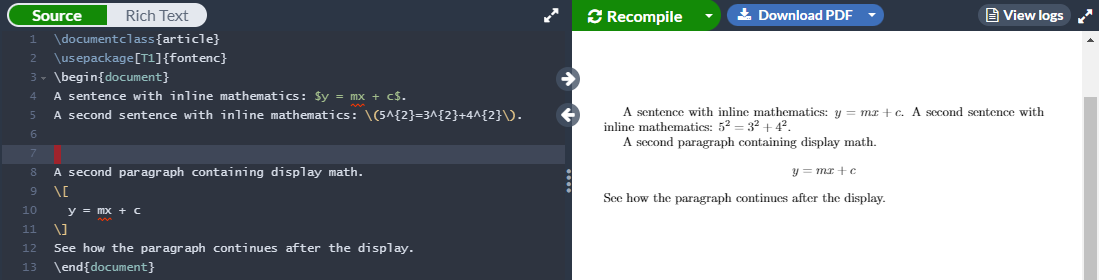
\includegraphics[width=0.9\linewidth]{day02-01A-inline-vs-display.png}
      \caption{Examples of inline vs. display math mo.}
      \label{fig:day02-01}
    \end{figure}
  \end{frame}

  \begin{frame}{Inline vs. Display Equations}
    Customary to write \emph{all} math symbols in math mode. For example,
    \begin{itemize} 
      \item $2$ and $-2$ (using inline math mode)
      \item 2 and -2 (without inline math mode)
    \end{itemize}
    Be careful about plaintext copied from other files that include:
    \begin{itemize}
      \item \$ (interpreted as math mode delimiter!)
      \item \_ (subscript symbol)
    \end{itemize}
  \end{frame}

  \begin{frame}{Mathematical Notation}
    Common mathematical constructs:
    \begin{itemize}
      \item Subscripts (\_) and superscripts ($\wedge$). Pay attention to curly braces ($\{\}$)!
      \item Specialist symbols (\texttt{\textbackslash sin}, \texttt{\textbackslash log}, \texttt{\textbackslash theta}, so many more!)
    \end{itemize}
    \begin{figure}
      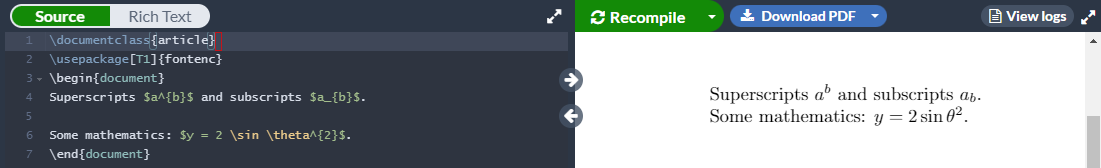
\includegraphics[width=1.0\linewidth]{day02-01B-symbols.png}
      \caption{Examples of mathematical symbols.}
      \label{fig:day02-01B}
    \end{figure}
  \end{frame}

  \begin{frame}{Display Mathematics}
    Display math environments are treated as part of a paragraph. Cannot end a paragraph (i.e., no newline within display environment).
    \begin{figure}
      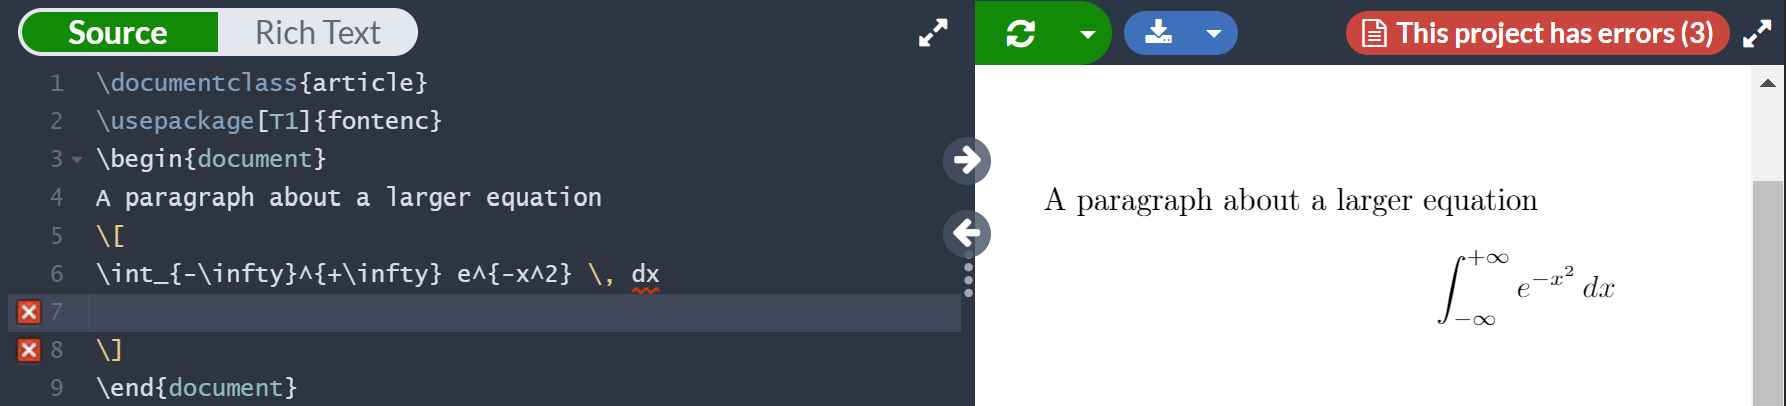
\includegraphics[width=1.0\linewidth]{day02-01C-error.png}
      \caption{Error arising from blank line in display math environment.}
      \label{fig:day02-01C}
    \end{figure}
  \end{frame}

  \begin{frame}{Display Mathematics}
    Whitespace delimited by specific control characters (e.g., \texttt{\textbackslash ,}).
    \begin{figure}
      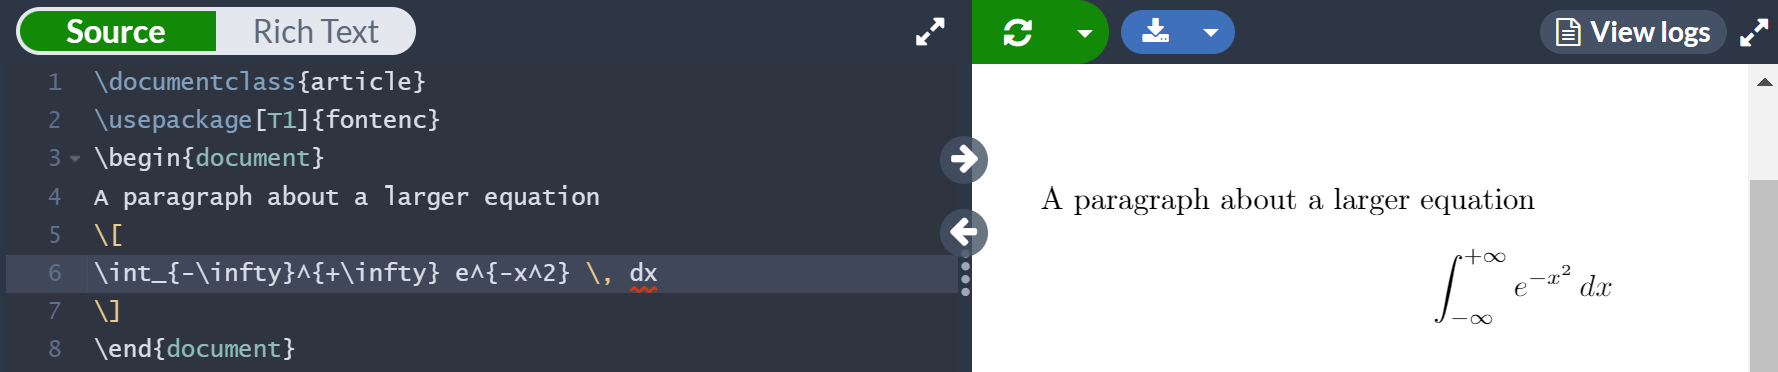
\includegraphics[width=1.0\linewidth]{day02-01D-whitespace.png}
      \caption{Whitespace in math environment requires control characters!}
      \label{fig:day02-01D}
    \end{figure}
  \end{frame}

  \begin{frame}{\texttt{equation} Environment}
    Numbered \texttt{equation} environments enable cross-referencing.
    \begin{figure}
      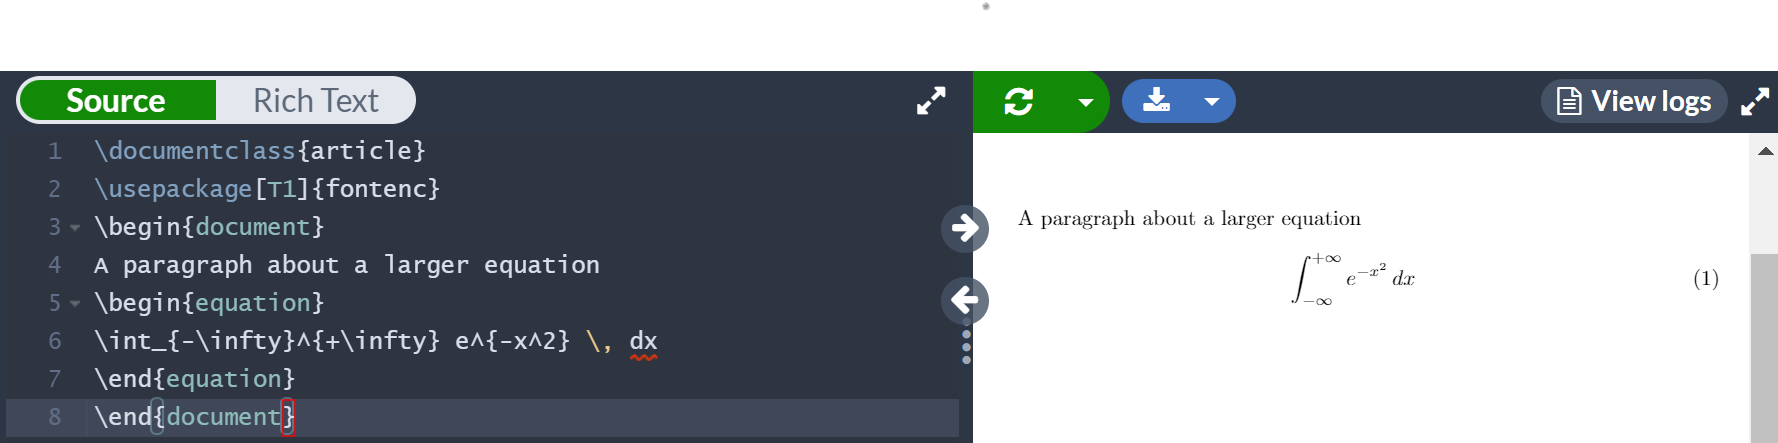
\includegraphics[width=1.0\linewidth]{day02-01E-numbered.png}
      \caption{Same math in \texttt{equation} environment}
      \label{fig:day02-01E}
    \end{figure}
  \end{frame}

  \begin{frame}{\texttt{align} Environment}
    To suppress numbers, add asterisk (*) 
    \begin{figure}
      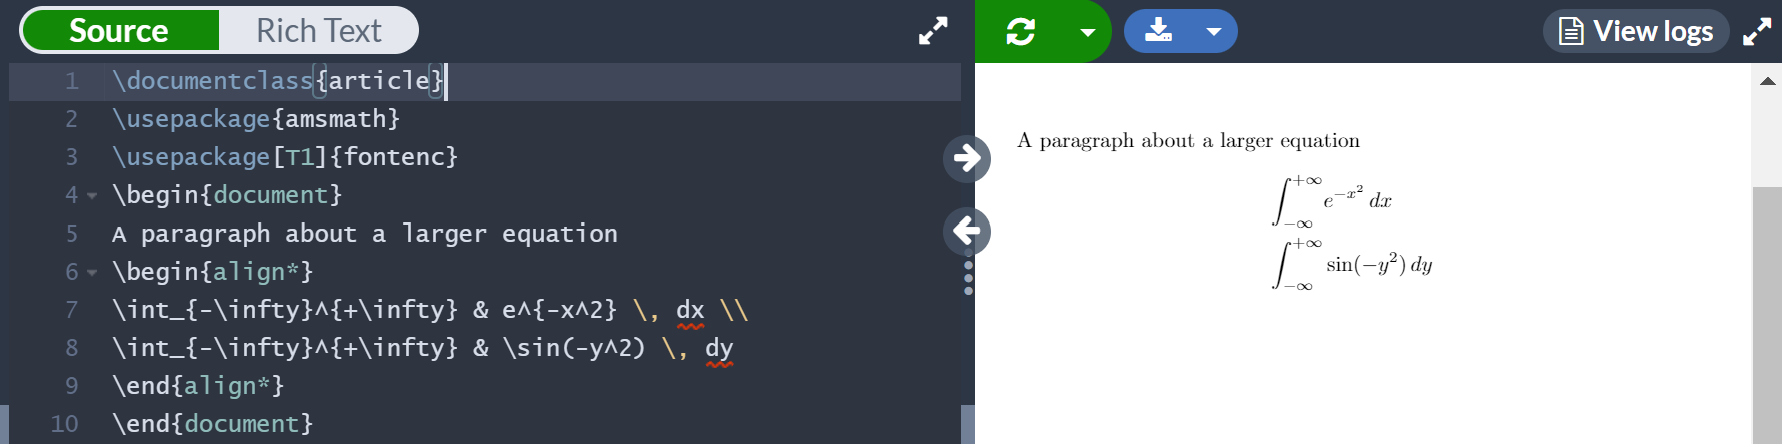
\includegraphics[width=1.0\linewidth]{day02-01G-asterisk.png}
      \caption{\texttt{align} environment with number suppressed.}
      \label{fig:day02-01G}
    \end{figure}
  \end{frame}

  \begin{frame}{\texttt{align} Environment}
    \texttt{align} environments also enable cross-referencing plus control of line alignment.
    \begin{itemize}
      \item \textbackslash\textbackslash : Force a newline
      \item \& : Location to align between two lines
    \end{itemize}
    \begin{figure}
      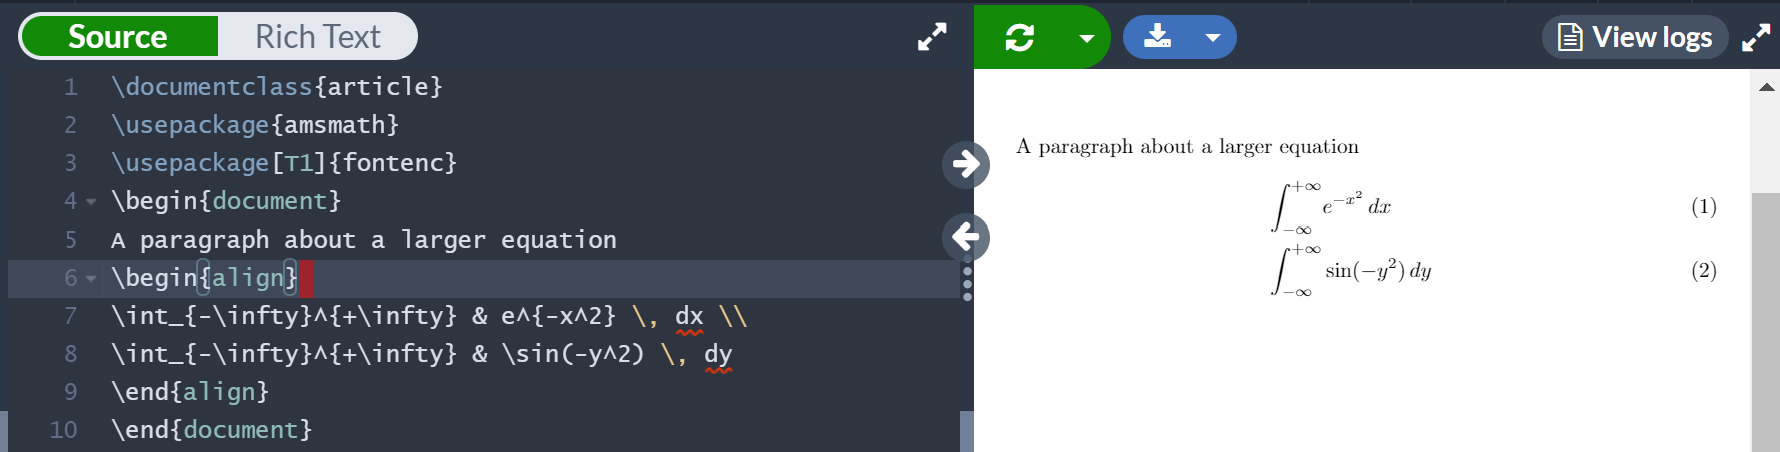
\includegraphics[width=1.0\linewidth]{day02-01F-align.png}
      \caption{Two lines in \texttt{align} environment}
      \label{fig:day02-01F}
    \end{figure}
  \end{frame}

  \begin{frame}{\texttt{align} Environment}
    To suppress number in \texttt{align} or \texttt{equation}, add an asterisk (i.e., \texttt{align*}, \texttt{equation*})
    \begin{figure}
      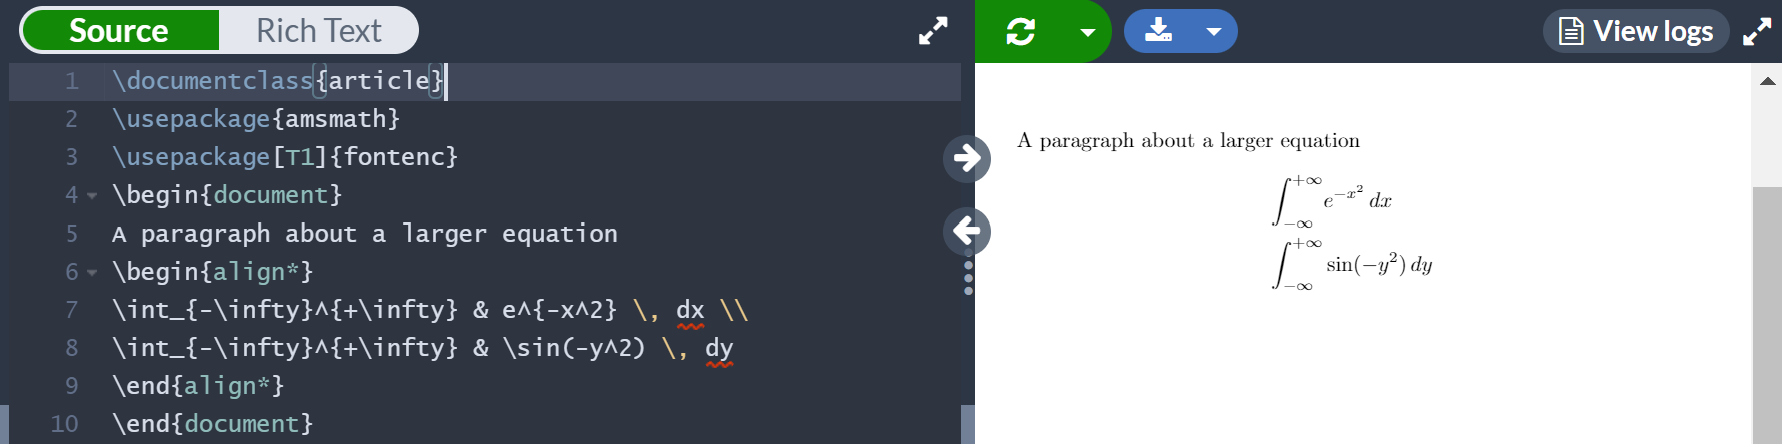
\includegraphics[width=1.0\linewidth]{day02-01G-asterisk.png}
      \caption{\texttt{align} without number.}
      \label{fig:day02-01G}
    \end{figure}
  \end{frame}

  \nofoot{
  \begin{frame}{Matrices}
    \texttt{amsmath} provides three matrix environments:
    \begin{enumerate}
      \item \texttt{matrix} -- Matrix with no brackets
      \item \texttt{pmatrix} -- Matrix with parentheses
      \item \texttt{bmatrix} -- Matrix with square brackets
    \end{enumerate}
    \begin{figure}
      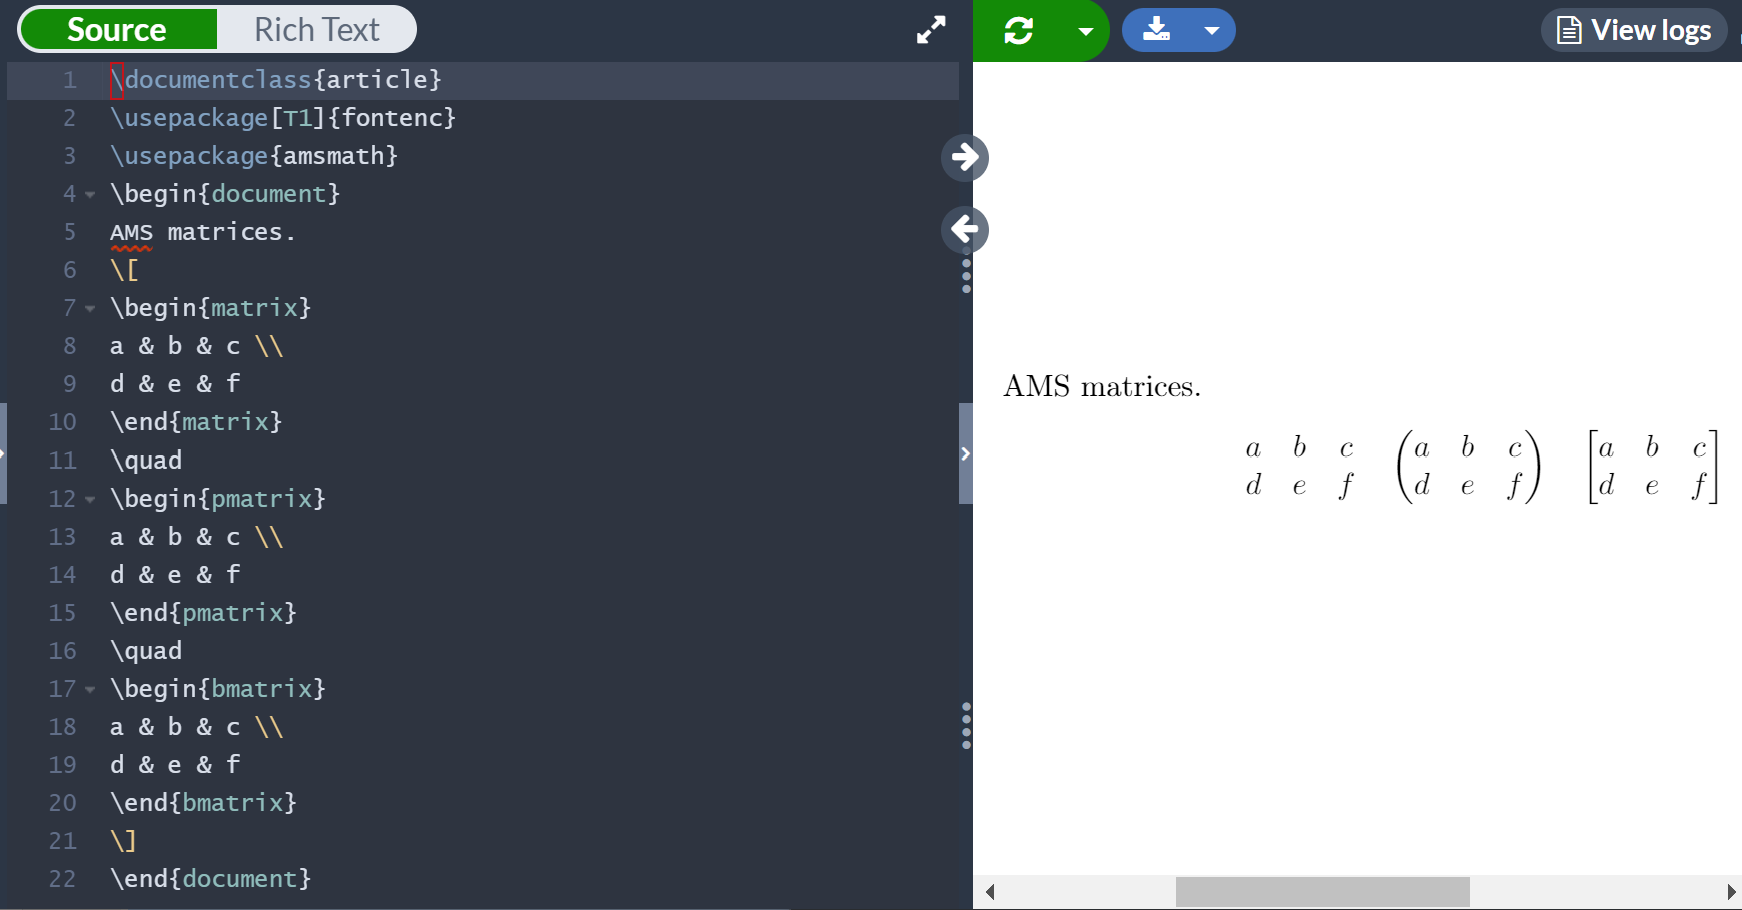
\includegraphics[width=0.8\linewidth]{day02-01H-matrices.png}
      \caption{Different matrices with different delimiters.}
      \label{fig:day02-01H}
    \end{figure}
  \end{frame}
  }

  \begin{frame}{Math Fonts}  
    Math fonts can convey specific meaning. Available math fonts are:
    \begin{table}
      \begin{tabular}{c|c|c}
        \textbf{Name} & \textbf{Command} & \textbf{Example} \\ \hline
        Roman & \texttt{\textbackslash mathrm} & $\mathrm{R}$ \\ \hline
        Italic & \texttt{\textbackslash mathit} & $\mathit{R}$ \\ \hline
        Boldface & \texttt{\textbackslash mathbf} & $\mathbf{R}$ \\ \hline
        Sans serif & \texttt{\textbackslash mathsf} & $\mathsf{R}$ \\ \hline
        Monospaced/typewriter & \texttt{\textbackslash mathtt} & $\mathtt{R}$ \\ \hline
        Double-struck/blackboard bold & \texttt{\textbackslash mathbb} & $\mathbb{R}$ 
      \end{tabular}
    \end{table}
  \end{frame}

  \begin{frame}{Normal Font}
    To use plain font in a math environment:
    \begin{itemize} 
      \item \textbackslash\texttt{text} to match outer font.
      \item \textbackslash\texttt{mathrm} roman font (regardless of outer font).
    \end{itemize}
    \begin{figure}
      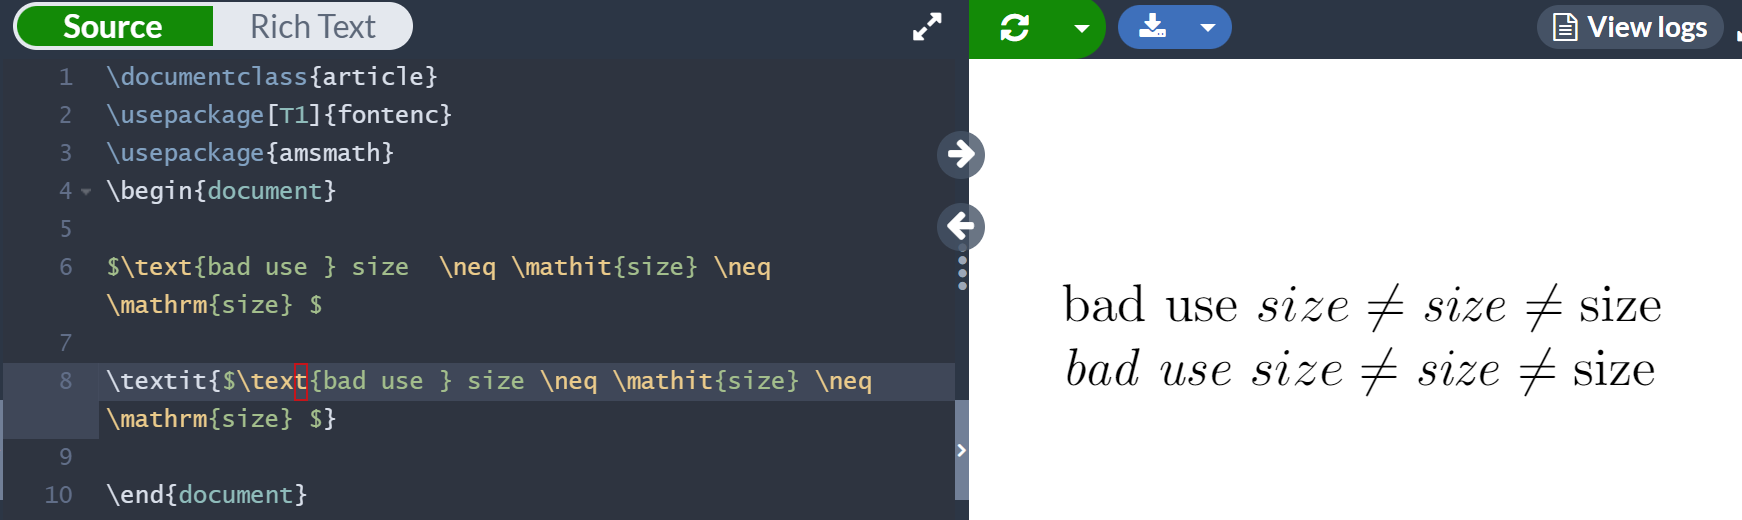
\includegraphics[width=0.8\linewidth]{day02-01I-plain.png}
      \caption{Plain font in math environment.}
      \label{fig:day02-01I}
    \end{figure}
  \end{frame}

  \begin{frame}{Searching for Symbols}
    So many math symbols! If you're lost, detexify (\texttt{http://detexify.kirelabs.org/classify.html}) can help.
    \begin{figure}
      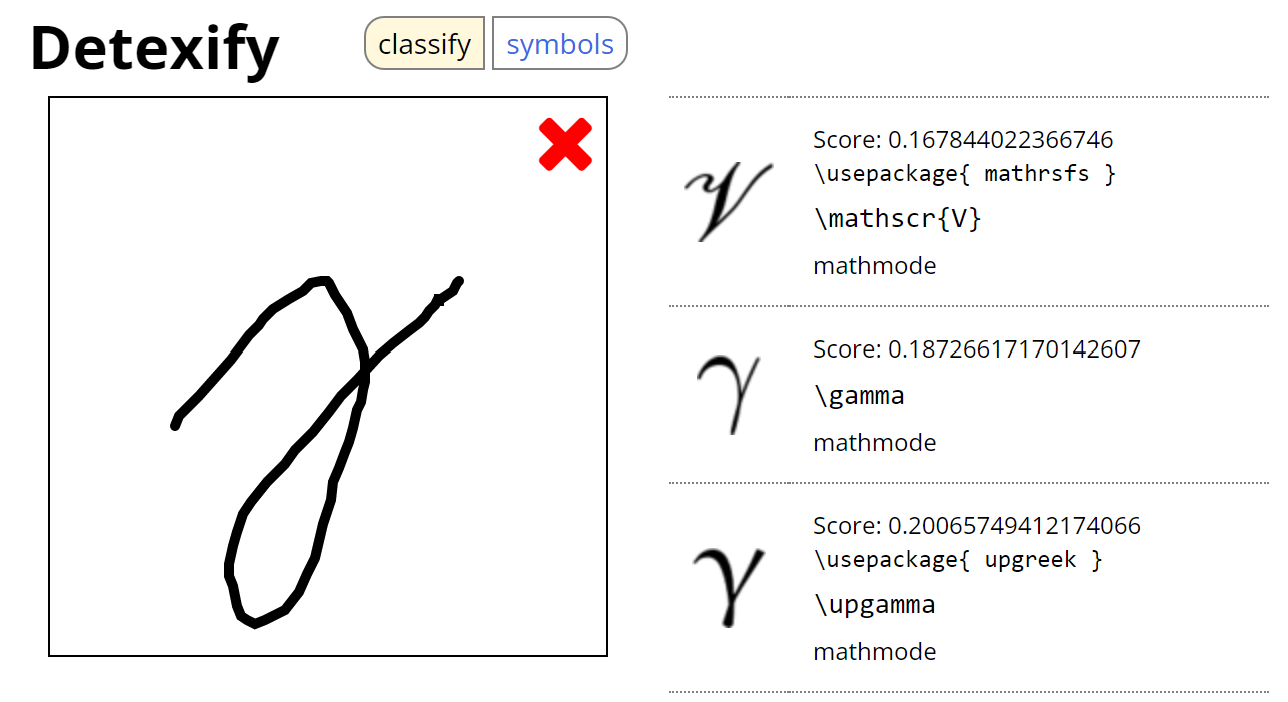
\includegraphics[width=0.8\linewidth]{day02-01J-detexify.png}
      \caption{Returned matches for a hand-drawn gamma ($\gamma$) symbol.}
      \label{fig:day02-01J}
    \end{figure}
  \end{frame}

\section{Fonts + Spacing}

  \begin{frame}[plain]
    \vfill
    \centering
    \begin{beamercolorbox}[sep=8pt,center,shadow=true,rounded=true]{Fonts + Spacing}
      \usebeamerfont{title}\insertsectionhead\par%
      \color{davisblue}\noindent\rule{10cm}{1pt} \\
      \footnotesize{Paragraph spacing, newlines, explicit spacing/formatting}
    \end{beamercolorbox}
    \vfill
  \end{frame}

  \begin{frame}{Paragraph Spacing}
    Behavior for new paragraphs:
    \begin{itemize}
      \item Default: indents, no blank line between paragraphs
      \item \texttt{parskip}: no indents, blank line between paragraphs
    \end{itemize}
    \begin{figure}
      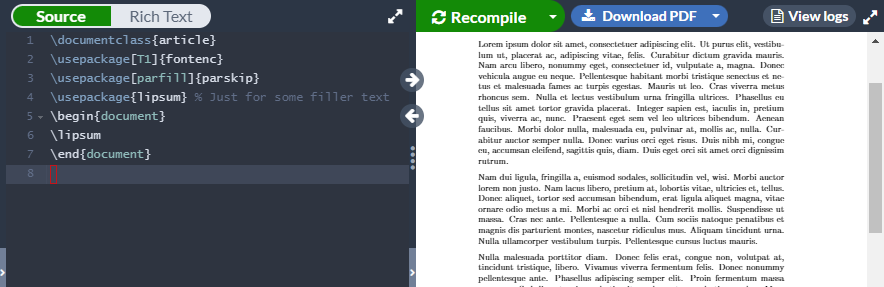
\includegraphics[width=0.8\linewidth]{day02-02A-parskip.png}
      \caption{New paragraph behavior using \texttt{parskip}.}
      \label{fig:day02-02A}
    \end{figure}
  \end{frame}

  \begin{frame}{Forcing Newlines}
    \begin{itemize}
      \item For default text, newlines between paragraphs should be automatically added by including `blank lines'
      \item In certain environments, need \textbackslash\textbackslash \, to force newlines
      \begin{itemize}
        \item End of \texttt{table} rows
        \item Inside of \texttt{center} environments
        \item Inside of \texttt{verse} environments (poetry)
      \end{itemize}
    \end{itemize}
  \end{frame}

  \begin{frame}{Explicit Whitespace}
    For more fine-tuned whitespace:
    \begin{itemize}
      \item \texttt{\textbackslash,} -- thin space (text mode)
      \item \texttt{\textbackslash.}, \texttt{\textbackslash:}, \texttt{\textbackslash;} -- different sized spaces (math mode)
      \item \texttt{\textbackslash hspace}, \texttt{\textbackslash vspace} -- explicit horizontal, vertical space
    \end{itemize}
    \begin{figure}
      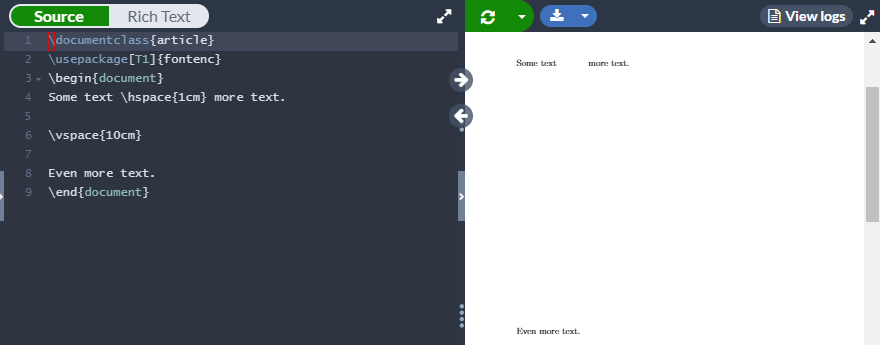
\includegraphics[width=0.8\linewidth]{day02-02B-explicit.png}
      \caption{Examples of \texttt{\textbackslash hspace}, \texttt{\textbackslash vspace}.}
      \label{fig:day02-02B}
    \end{figure}
  \end{frame}

  \begin{frame}{Explicit Text Formatting}
    For short pieces of text, the following formatting commands are available:
    \begin{table}
      \begin{tabular}{c|c|c}
        \textbf{Name} & \textbf{Command}               & \textbf{Example} \\ \hline
        Roman         & \texttt{\textbackslash textrm} & \textrm{Format} \\ \hline
        Italic        & \texttt{\textbackslash textit} & \textit{Format} \\ \hline
        Boldface      & \texttt{\textbackslash textbf} & \textbf{Format} \\ \hline
        Sans serif    & \texttt{\textbackslash textsf} & \textsf{Format} \\ \hline
        Monospaced    & \texttt{\textbackslash texttt} & \texttt{Format} \\ \hline
        Small caps    & \texttt{\textbackslash textsc} & \textsc{Format}
      \end{tabular}
    \end{table}
  \end{frame}

  \begin{frame}{Text Formatting Groups}
    \begin{itemize}
      \item Group $=$ anything in curly braces (\{\}). Use with large blocks of text.
      \item \texttt{\textbackslash itshape} and \texttt{\textbackslash bfseries} used to make groups italic and bold face, respectively.
    \end{itemize}
    \begin{figure}
      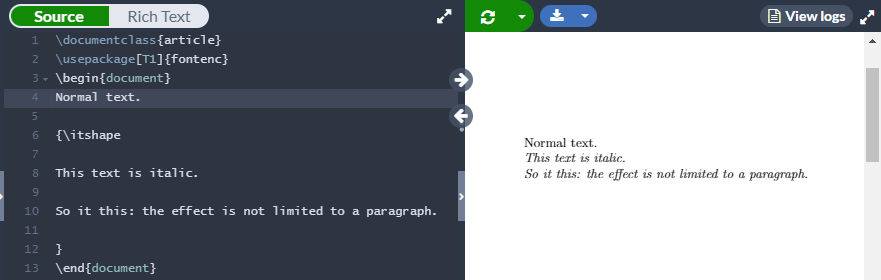
\includegraphics[width=0.8\linewidth]{day02-02C-groups.png}
      \caption{Example of \texttt{\textbackslash itshape} used with a group.}
      \label{fig:day02-02C}
    \end{figure}
  \end{frame}

  \begin{frame}{Font Sizes}
  \begin{itemize}
    \item Relative font size within a group -- \texttt{\textbackslash huge}, \texttt{\textbackslash large}, \texttt{\textbackslash normalsize}, \texttt{\textbackslash small}, \texttt{\textbackslash footnotesize}, \texttt{\textbackslash tiny}.
    \item \texttt{\textbackslash par} -- end of paragraph
  \end{itemize}
    \begin{figure}
      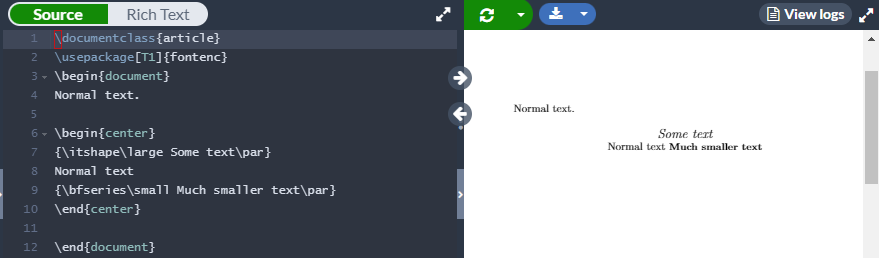
\includegraphics[width=0.8\linewidth]{day02-02D-fontsize.png}
      \caption{Example of \texttt{\textbackslash large}, \texttt{\textbackslash small} commands used with groups.}
      \label{fig:day02-02D}
    \end{figure}
  \end{frame}

\section{Citations + References}

  \begin{frame}[plain]
    \vfill
    \centering
    \begin{beamercolorbox}[sep=8pt,center,shadow=true,rounded=true]{Citations + References}
      \usebeamerfont{title}\insertsectionhead\par%
      \color{davisblue}\noindent\rule{10cm}{1pt} \\
      \footnotesize{\texttt{.bib} files, }
    \end{beamercolorbox}
    \vfill
  \end{frame}

  \nofoot{
  \begin{frame}{Reference Databases}
    Reference Databases (aka, bibliography files, \texttt{.bib} files) --
    \begin{itemize}
      \item Contain bibliography entries/references (e.g., \texttt{book}, \texttt{article}, etc.)
      \item Each entry contains multiple \emph{fields}.
      \item \texttt{author} field: contains all authors separated by \textbf{and} (important!).
    \end{itemize}
    \begin{figure}[thp]
      \centering
      \begin{tabular}{c}
        \lstinputlisting[linewidth=\linewidth, language=TeX, basicstyle=\ttfamily\tiny, tabsize=1, boxpos=c, firstline=1, lastline=7]{example.bib}
      \end{tabular}
      \caption{Example \text{.bib} entry.}
    \end{figure}
    \blfootnote{\bibentry{oetiker1995not}}
  \end{frame}
  }

  \begin{frame}{Using Databases in \LaTeX}
    Behind the scenes, three steps:
    \begin{enumerate}
      \item Compile document; creates list of cited references in document (not always everything in the database!).
      \item Run a program (BibTeX or Biber); takes cited references, matches them to database entries, puts them in order.
      \item Compile document again; resolves citations in document.
    \end{enumerate}
    \textbf{Note}: Overleaf will abstract out this process. Only need to hit ``Compile.''
  \end{frame}

  \begin{frame}{Create a Database}
    \begin{figure}
      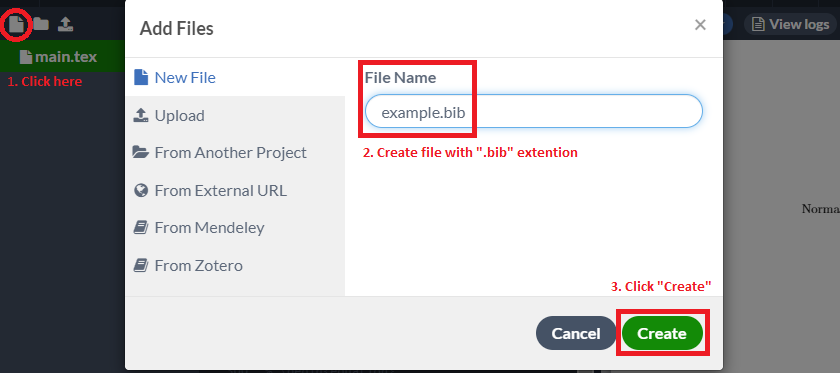
\includegraphics[width=0.8\linewidth]{day02-03A-database.png}
      \caption{Creating a new \texttt{.bib} file in Overleaf.}
      \label{fig:day02-03A}
    \end{figure}
  \end{frame}

  \begin{frame}{Add an Entry}
    \begin{figure}
      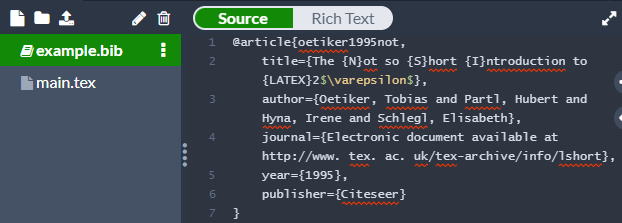
\includegraphics[width=0.8\linewidth]{day02-03B-entry.png}
      \caption{\texttt{.bib} file with a single entry.}
      \label{fig:day02-03B}
    \end{figure}
  \end{frame}

  \begin{frame}{BibTeX with \texttt{natbib}}
    \begin{itemize}
      \item Using \texttt{natbib} package (BibTeX-based)
      \item Parenthetical citation (\texttt{\textbackslash citep}) vs. Textual citation (\texttt{\textbackslash citet})
    \end{itemize}
    \begin{figure}
      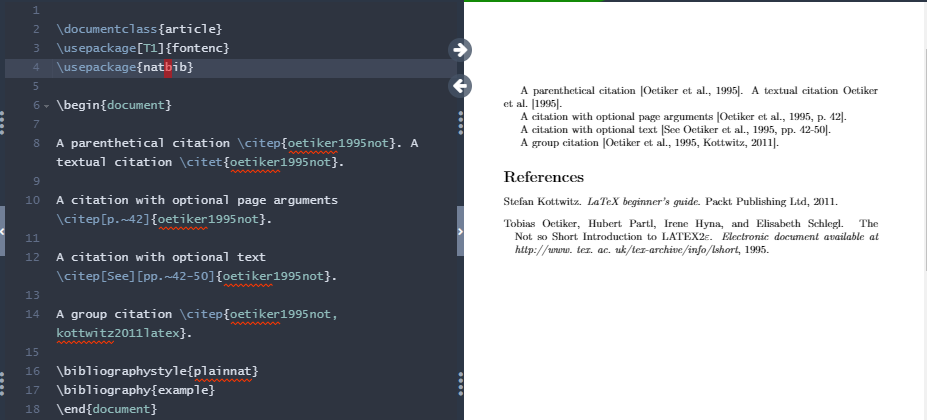
\includegraphics[width=0.8\linewidth]{day02-03C-natbib.png}
      \caption{Textual vs. parenthetical citations using \texttt{natbib}.}
      \label{fig:day02-03C}
    \end{figure}
  \end{frame}

\begin{frame}{End of Day 02}
  \begin{itemize}
    \item Finished: Lessons 1-6 (Day 01) and 7-12 (Day 02) from \texttt{learnlatex.org}
    \item Lessons 13 to 16 -- can ask questions re: these on the Slack channel! (\#latex101)
    \item Next time: Resume/CV templates, Beamer
  \end{itemize}
\end{frame}

\begin{frame}{References}
  \bibliographystyle{ieeetr}
  \bibliography{example}
\end{frame}

} %end footnotsize

\end{document}
